% !TEX root = task-2-12-1.tex
% Editable task bank. Append new BankTask blocks at the end of the document.
\documentclass[12pt,a4paper]{article}
\usepackage{physics-textbook}
\usepackage{graphicx,needspace}
\usetikzlibrary{decorations.pathmorphing}
\newif\ifShowSolutions
\ifdefined\TutorEdition
  \ShowSolutionstrue
\else
  \ShowSolutionsfalse % Change to \ShowSolutionstrue to display solutions.
\fi
\newcounter{banktask}
\newsavebox{\BankTaskBox}
\newcommand{\BankTaskContent}[3]{%
  \noindent\textbf{\thebanktask.}\quad #2\par
  \ifShowSolutions
    \Needspace{50mm}% Keep the solution heading with its opening text or diagram.
    #3\par
    \ifdefined\TutorEdition
      \ifcsname TutorSource#1\endcsname
        \nopagebreak\smallskip{\small\csname TutorSource#1\endcsname\par}%
      \fi
    \fi
  \fi
}
\newcommand{\BankTask}[3]{%
  \refstepcounter{banktask}\par\medskip
  \sbox{\BankTaskBox}{\begin{minipage}{\linewidth}%
    \BankTaskContent{#1}{#2}{#3}\end{minipage}}%
  \ifdim\dimexpr\ht\BankTaskBox+\dp\BankTaskBox\relax>\dimexpr\textheight-20mm\relax
    \Needspace{35mm}\BankTaskContent{#1}{#2}{#3}%
  \else
    \Needspace{\dimexpr\ht\BankTaskBox+\dp\BankTaskBox\relax}%
    \noindent\usebox{\BankTaskBox}\par
  \fi
  \medskip
}
\begin{document}
\BookSubsection{2.12.1}{Тепловые двигатели и КПД}


% Source sdamgia-1113: https://phys-ege.sdamgia.ru/problem?id=1113
\BankTask{sdamgia-1113}{
Идеальная тепловая машина за цикл работы получает от нагревателя $100\,\text{Дж}$ и отдает холодильнику $40\,\text{Дж}$. Каков КПД тепловой машины? ((В процентах.))
}{
\smallskip\noindent\textbf{Решение}\par
КПД тепловой машины связано с количеством теплоты, полученным за цикл от нагревателя, и количеством теплоты, отданным холодильнику, соотношением: 

$\eta = ( 1 - \frac{Q_2}{Q_1} ) \cdot 100\%= ( 1 - \frac{40\text{Дж}}{100\text{Дж}} ) \cdot 100\%=60\%.$

Ответ: $60$.
}

% Source sdamgia-1117: https://phys-ege.sdamgia.ru/problem?id=1117
\BankTask{sdamgia-1117}{
Идеальная тепловая машина с КПД $20$\% за цикл работы отдает холодильнику $80\,\text{Дж}$. Какую полезную работу машина совершает за цикл? ((В джоулях.))
}{
\smallskip\noindent\textbf{Решение}\par
КПД тепловой машины связано с количеством теплоты $Q_1,$ полученным от нагревателя, и полезной работой $A$ за цикл соотношением $\eta = \frac{A}{Q_1} \cdot 100\%.$ Принимая во внимание связь $Q_1$ и $A$ с количеством теплоты $Q_2,$ отданным холодильнику за цикл, $Q_1=A + Q_2,$ получаем:

$\eta= \frac{A}{A + Q_2} \cdot 100\% \Longleftrightarrow \eta A + \eta Q_2=A \cdot 100\% \Longleftrightarrow \eta Q_2=A ( 100\% - \eta ) \Longleftrightarrow$

$\Longleftrightarrow A= \frac{\eta Q_2}{100\% - \eta} = \frac{20\% \cdot 80\text{Дж}}{100\% - 20\%} =20\text{Дж}.$

Ответ: $20$.
}

% Source sdamgia-1120: https://phys-ege.sdamgia.ru/problem?id=1120
\BankTask{sdamgia-1120}{
Идеальная тепловая машина с КПД $60$\% за цикл работы получает от нагревателя $50\,\text{Дж}$. Какое количество теплоты машина отдает за цикл холодильнику? ((В джоулях.))
}{
\smallskip\noindent\textbf{Решение}\par
КПД тепловой машины связано с количеством теплоты, полученным за цикл от нагревателя, и количеством теплоты, отданным холодильнику, соотношением $\eta = ( 1 - \frac{Q_2}{Q_1} ) \cdot 100\%.$ Отсюда находим, что количество теплоты, которое машина отдает за цикл холодильнику, равно:

$Q_2=Q_1 ( 1 - \frac{\eta}{100\%} ) =50\text{Дж} \cdot ( 1 - \frac{60\%}{100\%} ) =20\text{Дж}.$

Ответ: $20$.
}

% Source sdamgia-9146: https://phys-ege.sdamgia.ru/problem?id=9146
\BankTask{sdamgia-9146}{
В некотором циклическом процессе модуль количества теплоты, отданного газом за один цикл холодильнику, в $21/9$ раза больше, чем совершаемая газом за цикл работа. Чему равен КПД такого теплового двигателя? (В процентах.)
}{
\smallskip\noindent\textbf{Решение}\par
КПД теплового двигателя равно $\eta= \frac{A}{Q_1} \cdot 100\%,$ где $A$ — совершаемая газом работа, $Q_{1}$ — теплота, даваемая газу нагревателем. $A=Q_1 - Q_2,$ где $Q_{2}$ — теплота, отдаваемая газом холодильнику, по условию $Q_2 = \frac{21}{9} A.$ Найдем КПД теплового двигателя:

$\eta = \frac{A}{A + Q_2} \cdot 100\%= \frac{A}{A + \frac{21}{9} A} \cdot 100\%= \frac{9}{30} \cdot 100\%=30\%.$

Ответ: $30$.
}

% Source sdamgia-10314: https://phys-ege.sdamgia.ru/problem?id=10314
\BankTask{sdamgia-10314}{
В топке паровой машины сгорело $50\,\text{кг}$ каменного угля, удельная теплота сгорания которого равна $30\,\text{МДж}$/кг. При этом машиной была совершена полезная механическая работа $135\,\text{МДж}$. Чему равен КПД этой тепловой машины? (В процентах.)
}{
\smallskip\noindent\textbf{Решение}\par
В процессе сгорания выделилось тепло:

$Q=qm=1500\text{МДж}.$

КПД определяется как отношение полезной работы к затраченной энергии:

$\eta = \frac{A}{Q} = \frac{135}{1500} =0{,}09.$ 

Таким образом, КПД тепловой машины равен $9$\%.

Ответ: $9$.
}

% Source sdamgia-23232: https://phys-ege.sdamgia.ru/problem?id=23232
\BankTask{sdamgia-23232}{
Идеальная тепловая машина, обладающая КПД $10$ \%, использует в качестве холодильника резервуар со льдом при температуре $0^\circ$C. За один цикл работы этой машины в холодильнике тает $900\,\text{г}$ льда. Какое количество теплоты потребляет эта машина от нагревателя за один цикл работы? (В килоджоулях.)
}{
\smallskip\noindent\textbf{Решение}\par
КПД тепловой машины равно $\eta = 1 - \frac{Q_{\text{x}}}{Q_{\text{н}}} ,$ откуда теплота, отданная нагревателем, равна $Q_{\text{н}}= \frac{Q_{\text{x}}}{1 - \eta} .$ Для плавления льда холодильник получает количество теплоты $Q=\lambda m.$ Тогда теплота, отданная нагревателем, равна:

$Q_{\text{н}}= \frac{\lambda m}{1 - \eta} = \frac{3{,}3 \cdot 10 ^{5} \cdot 0{,}9}{1 - 0{,}1} =330\text{кДж}.$

Ответ: $330$.
}

% Source sdamgia-32755: https://phys-ege.sdamgia.ru/problem?id=32755
\BankTask{sdamgia-32755}{
За $4$ цикла своей работы тепловой двигатель совершил работу $120\,\text{кДж}$. Какое количество теплоты газ отдает холодильнику за один цикл, если КПД двигателя равен $60$\%? (В килоджоулях.)
}{
\smallskip\noindent\textbf{Решение}\par
За один цикл газ совершил работу $30\,\text{кДж}$. Из формулы для КПД теплового двигателя $\eta= \frac{A}{Q_1}$ и формулы $A=Q_1 - Q_2$ выразим количество теплоты, отданное газом холодильнику за один цикл:

$Q_2= \frac{( 1 - \eta ) A}{\eta} = \frac{( 1 - 0{,}6 ) \cdot 30}{0{,}6} =20\text{кДж}.$

Ответ: $20$.
}

% Source sdamgia-50819: https://phys-ege.sdamgia.ru/problem?id=50819
\BankTask{sdamgia-50819}{
\begin{center}\begin{tikzpicture}[task graph,>=stealth]\draw[->](0,0)--(5,0)node[below]{\(V\)};\draw[->](0,0)--(0,3.7)node[left]{\(p\)};\node[below left]at(0,0){\(0\)};\fill(0.7,2.85)circle(1.25pt)node[above left]{\(1\)};\fill(2.75,2.85)circle(1.25pt)node[above right]{\(2\)};\fill(2.75,0.8)circle(1.25pt)node[right]{\(3\)};\draw(0.7,2.85)--(2.75,2.85);\draw[->](0.7,2.85)--(1.971,2.850);\draw(2.75,2.85)--(2.75,0.8);\draw[->](2.75,2.85)--(2.750,1.579);\draw(2.75,.8)..controls(1.7,.83)and(.77,1.4)..(.7,2.85);\draw[->](1.53,1.23)--(1.3,1.45);\end{tikzpicture}\end{center}
В качестве рабочего тела в тепловой машине используется идеальный одноатомный газ, который совершает циклический процесс, состоящий из изобарного нагревания ($1$ → $2$), изохорного охлаждения ($2$ → $3$) и адиабатного сжатия ($3$ → $1$). Отношение работы $A_{12}$, совершённой газом в изобарном процессе, к работе $A'_{31},$ совершённой над газом при адиабатном сжатии равно $2$. Определите КПД этой тепловой машины.
}{
\smallskip\noindent\textbf{Решение}\par
Проанализируем процессы. В изобарном процессе $1$–$2$ объем увеличивается. По закону Гей  — Люссака $\frac{V}{T} = const$ при увеличении объема увеличивается абсолютная температура газа. 
Работа газа в этом процессе равна $A_{12}=\nu R ( T_2 - T_1 )$ положительна, изменение внутренней энергии одноатомного газа $\Delta U_{12}= \frac{3}{2} \nu R ( T_2 - T_1 )$ положительно. Тогда по первому закону термодинамики $Q_{12}=A_{12} + \Delta U_{12}$ положительно и равно $Q_{12}= \frac{5}{2} \nu R ( T_2 - T_1 ) = \frac{5}{2} A_{12} .$ Значит, газ в этом процессе получает теплоту.
В изохорном процессе $2$–$3$ газ работу не совершает. Согласно закону Шарля $\frac{p}{T} = const$ при уменьшении давления уменьшается абсолютная температура газа. Следовательно, внутренняя энергия газа уменьшается, а по первому закону термодинамики $Q_{23}=\Delta U_{23}$ количество теплоты отрицательно, газ теплоту отдает.
В адиабатном процессе $3$–$1$ газ не получает и не отдает теплоту $Q_{31}=0,$ газ сжимается и поэтому совершает отрицательную работу, модуль которой по условию $|A_{31}|= \frac{A_{12}}{2} .$
Таким образом, работа газа за цикл равна $A=A_{12} + A_{31}= \frac{A_{12}}{2} .$ 
Количество теплоты, полученное газом за цикл $Q=Q_{12}= \frac{5}{2} A_{12} .$
Находим КПД цикла:

\[\eta= \frac{A}{Q} = \frac{2A_{12}}{2 \cdot 5A_{12}} =0{,}2=20\%.\]

Ответ: $20$\%.
}

% Source sdamgia-24380: https://phys-ege.sdamgia.ru/problem?id=24380
\BankTask{sdamgia-24380}{
\begin{center}\begin{tikzpicture}[task graph,>=stealth]\draw[->](0,0)--(5,0)node[below]{\(T\)};\draw[->](0,0)--(0,3.7)node[left]{\(p\)};\node[below left]at(0,0){\(0\)};\fill(1,1.4)circle(1.25pt)node[above left]{\(1\)};\fill(2,2.8)circle(1.25pt)node[above left]{\(2\)};\fill(4,2.8)circle(1.25pt)node[above right]{\(3\)};\fill(2,1.4)circle(1.25pt)node[right]{\(4\)};\draw(1,1.4)--(2,2.8);\draw[->](1,1.4)--(1.620,2.268);\draw(2,2.8)--(4,2.8);\draw[->](2,2.8)--(3.240,2.800);\draw(4,2.8)--(2,1.4);\draw[->](4,2.8)--(2.760,1.932);\draw(2,1.4)--(1,1.4);\draw[->](2,1.4)--(1.380,1.400);\draw[thin](0,0)--(1,1.4)(0,0)--(2,1.4)(1,0)--(1,1.4)(2,0)--(2,2.8)(4,0)--(4,2.8);\node[below]at(1,0){\(T_1\)};\node[below]at(2,0){\(T_2=T_4=2T_1\)};\node[below]at(4,0){\(T_3\)};\end{tikzpicture}\end{center}
В тепловом двигателе $1$ моль одноатомного разреженного газа совершает цикл $1$−$2$−$3$−$4$−$1$, показанный на графике в координатах p–T, где p  — давление газа, Т  — абсолютная температура. Температуры в точках $2$ и $4$ равны и превышают температуру в точке $1$ в $2$ раза. Определите КПД цикла.
}{
\smallskip\noindent\textbf{Решение}\par
$1$.  Рассмотрим процессы, происходящие на каждом участке: 
На участке $1$−$2$ происходит изохорное нагревание ($V_{1}$  =  $V_{2}$), при котором по графику температура увеличивается в $2$ раза. Значит, исходя из закона $\frac{p_2}{p_1} = \frac{T_2}{T_1} ,$ давление увеличивается в $2$ раза. 
На участке $2$−$3$ происходит изобарное нагревание, при котором по закону $\frac{V_3}{V_2} = \frac{T_3}{T_2}$ или $\frac{V_3}{V_1} = \frac{T_3}{2T_1} .$
На участке $3$−$4$ происходит изохорное охлаждение, при котором по закону $\frac{p_4}{p_3} = \frac{T_4}{T_3}$ или $\frac{p_4}{2p_1} = \frac{2T_1}{T_3} .$
На участке $4$−$1$ происходит изобарное охлаждение. Тогда в предыдущем уравнении $\frac{p_1}{2p_1} = \frac{2T_1}{T_3} ,$ откуда $T_{3}$  =  $4$T$_{1}$.
$2$.  Найдем работу газа за цикл. На участках $1$−$2$ и $3$−$4$ объемы не меняются, поэтому работа не совершается. Следовательно, работы за цикл равна:

A  =  $A_{2-3}$ + $A_{4-1}$,
$A_2 - 3= \nu R ( T_3 - T_2 ) ;$ $R ( 4T_1 - 2T_1 ) =2\nu RT_1$
$A_4 - 1=\nu R ( T_1 - T_4 ) = - \nu RT_1$
$A=\nu RT_1.$

$3$.  Газ получает теплоту на участках $1$–$2$ и $2$–$3$. Найдем количество теплоты на каждом участке, применив первый закон термодинамики:

$Q_1 - 2=\Delta U_1 - 2= \frac{3}{2} \nu R ( T_2 - T_1 ) =1{,}5\nu RT_1,$
$Q_2 - 3=\Delta U_2 - 3 + A_2 - 3= \frac{3}{2} \nu R ( T_3 - T_2 ) + \nu R ( T_3 - T_2 ) = \frac{5}{2} \nu R ( 4T_1 - 2T_1 ) =5\nu RT_1,$
$Q_{\,\text{пол}}=Q_1 - 2 + Q_2 - 3=6{,}5\nu RT_1.$

$4$.  Найдем КПД циклического процесса:

\[\eta= \frac{A}{Q_{\,\text{пол}}} = \frac{\nu RT_1}{6{,}5\nu RT_1} = \frac{1}{6{,}5} \approx15\%.\]

Ответ: $15$\%.
}

% Source sdamgia-42652: https://phys-ege.sdamgia.ru/problem?id=42652
\BankTask{sdamgia-42652}{
\begin{center}\begin{tikzpicture}[task graph,>=stealth]\draw[->](0,0)--(5,0)node[below]{\(V\)};\draw[->](0,0)--(0,3.7)node[left]{\(p\)};\node[below left]at(0,0){\(0\)};\fill(1.2,0.35)circle(1.25pt)node[right]{\(1\)};\fill(1.2,1.6)circle(1.25pt)node[above left]{\(2\)};\fill(3.7,3.15)circle(1.25pt)node[above right]{\(3\)};\draw(1.2,0.35)--(1.2,1.6);\draw[->](1.2,0.35)--(1.200,1.125);\draw(1.2,1.6)--(3.7,3.15);\draw[->](1.2,1.6)--(2.750,2.561);\draw(3.7,3.15)--(1.2,0.35);\draw[->](3.7,3.15)--(2.150,1.414);\foreach \y/\i/\x in {.35/1/1.2,1.6/2/1.2,3.15/3/3.7}{\draw[dashed](0,\y)--(\x,\y);\node[left]at(0,\y){\(p_{\i}\)};}\draw[dashed](1.2,0)--(1.2,.35)(3.7,0)--(3.7,3.15);\node[below]at(1.2,0){\(V_1\)};\node[below]at(3.7,0){\(V_3\)};\end{tikzpicture}\end{center}
На рисунке в координатах p–V представлен циклический процесс, проводимый с идеальным одноатомным газом. Давление идеального одноатомного газа изохорно увеличивают в $4$ раза, затем объём газа увеличивают в $2{,}5$ раза так, что давление линейно зависит от объёма и возрастает в $2$ раза. После этого газ возвращают в исходное состояние в процессе, в котором давление линейно зависит от объёма. Масса газа постоянна. Определите коэффициент полезного действия теплового двигателя, работающего по этому циклу.
}{
\smallskip\noindent\textbf{Решение}\par
Проанализируем процессы, происходящие с идеальным газом. На участке $1$−$2$ давление газа изохорно увеличивается. Следовательно, согласно закону Шарля $\frac{p}{T} =const$ его температура также увеличивается. Тогда газ не совершает работу, его внутренняя энергия увеличивается. По первому закону термодинамики $Q=A + \Delta U > 0,$ то есть газ теплоту получает.
На участке $2$−$3$ и объем, и давление увеличиваются прямо пропорционально, следовательно, температура увеличивается. Таким образом, работа газа положительна, внутренняя энергия увеличивается, газ теплоту получает.
На участке $3$−$1$ объем газа уменьшается в $2{,}5$ раза, давление уменьшается в $8$ раз, следовательно, температура уменьшается. Значит, работа газа отрицательна, внутренняя энергия уменьшается, газ теплоту отдает.
В результате анализа процессов делаем вывод, что газ получает теплоту на участках $1$−$2$ и $2$−$3$. Найдем это количество теплоты.
Для участка $1$−$2$ по первому закону термодинамики 

\[Q_{12}=\Delta U_{12}= \frac{3}{2} ( p_2 - p_1 ) V_1= \frac{3}{2} ( 4p_1 - p_1 ) V_1=4{,}5p_1V_1.\]

Найдем работу, изменение внутренней энергии и полученное количество теплоты на участке $2$−$3$:

$A_{23}= \frac{p_2 + p_3}{2} ( V_3 - V_1 ) = \frac{4p_1 + 8p_1}{2} ( 2{,}5V_1 - V_1 ) =9p_1V_1;$
$\Delta U_{23}=U_3 - U_2= \frac{3}{2} ( p_3V_3 - p_2V_2 ) = \frac{3}{2} ( 8p_1 \cdot 2{,}5V_1 - 4p_1V_1 ) =24p_1V_1;$
$Q_{23}=\Delta U_{23} + A_{23}=9p_1V_1 + 24p_1V_1=33p_1V_1.$

Таким образом, за цикл идеальный газ получил количество теплоты

\[Q=Q_{12} + Q_{23}=4{,}5p_1V_1 + 33p_1V_1=37{,}5p_1V_1.\]

Работу газа за цикл найдем как площадь треугольника под графиком:

\[A= \frac{( p_2 - p_1 ) ( V_3 - V_1 )}{2} = \frac{( 4p_1 - p_1 ) ( 2{,}5V_1 - V_1 )}{2} =2{,}25p_1V_1.\]

Тогда КПД цикла

\[\eta= \frac{A}{Q} \cdot 100\%= \frac{2{,}25p_1V_1}{37{,}5p_1V_1} \cdot 100\% = 6\%.\]

Ответ: $6$\%.
}


% Source 4EF342: https://ege.fipi.ru/bank/questions.php?search=1&proj=BA1F39653304A5B041B656915DC36B38&qid=4EF342
\BankTask{4EF342}{
Рабочее тело тепловой машины за цикл получает от нагревателя количество теплоты, равное \(100\,\text{Дж}\), и совершает работу \(60\,\text{Дж}\). Каков КПД тепловой машины (в $\%$)?
}{
\smallskip\noindent\textbf{Решение от GPT}\par
КПД тепловой машины:
\[
\eta=\frac{A}{Q_1}=\frac{60}{100}=0{,}6=60\%.
\]
Ответ: \(60\%\).
}

% Source 81C4BA: https://ege.fipi.ru/bank/questions.php?search=1&proj=BA1F39653304A5B041B656915DC36B38&qid=81C4BA
\BankTask{81C4BA}{
Рабочее тело тепловой машины с КПД \(30\%\) за цикл работы отдаёт холодильнику количество теплоты, равное \(70\,\text{Дж}\). Какое количество теплоты за цикл рабочее тело получает от нагревателя (в $\text{Дж}$)?
}{
\smallskip\noindent\textbf{Решение от GPT}\par
Из \(\eta=1-\dfrac{Q_2}{Q_1}\) получаем
\[
Q_1=\frac{Q_2}{1-\eta}=\frac{70}{1-0{,}30}=100\,\text{Дж}.
\]
Ответ: \(100\,\text{Дж}\).
}

% Source C2BD49: https://ege.fipi.ru/bank/questions.php?search=1&proj=BA1F39653304A5B041B656915DC36B38&qid=C2BD49
\BankTask{C2BD49}{
Тепловая машина с КПД $30\%$ за цикл работы получает от нагревателя количество теплоты, равное $120\,\text{Дж}$. Какую работу машина совершает за цикл (в $\text{Дж}$)?
}{
\smallskip\noindent\textbf{Решение от GPT}\par
$\eta=A/Q_1$, поэтому $A=\eta Q_1=0{,}30\cdot120=36\,\text{Дж}$. Ответ: $36\,\text{Дж}$.
}

% Source 80CCD9: https://ege.fipi.ru/bank/questions.php?search=1&proj=BA1F39653304A5B041B656915DC36B38&qid=80CCD9
\BankTask{80CCD9}{
Рабочее тело теплового двигателя за цикл совершает работу, равную $15\,\text{кДж}$, и получает от нагревателя количество теплоты, равное $75\,\text{кДж}$. Какое количество теплоты рабочее тело отдаёт холодильнику за цикл (в $\text{кДж}$)?
}{
\smallskip\noindent\textbf{Решение от GPT}\par
За цикл $\Delta U=0$, поэтому $Q_1=A+Q_2$. Отданная холодильнику теплота $Q_2=75-15=60\,\text{кДж}$. Ответ: $60\,\text{кДж}$.
}

% Source D1C429: https://ege.fipi.ru/bank/questions.php?search=1&proj=BA1F39653304A5B041B656915DC36B38&qid=D1C429
\BankTask{D1C429}{
Рабочее тело тепловой машины за один цикл отдаёт холодильнику количество теплоты $100\,\text{Дж}$ и совершает работу $30\,\text{Дж}$. Какое количество теплоты получает рабочее тело от нагревателя за два цикла (в $\text{Дж}$)?
}{
\smallskip\noindent\textbf{Решение от GPT}\par
За один цикл $Q_1=Q_2+A=100+30=130\,\text{Дж}$. За два цикла $Q=2Q_1=260\,\text{Дж}$. Ответ: $260\,\text{Дж}$.
}

% Source B44BA2: https://ege.fipi.ru/bank/questions.php?search=1&proj=BA1F39653304A5B041B656915DC36B38&qid=B44BA2
\BankTask{B44BA2}{
Тепловая машина с КПД $20\%$ совершает за цикл работу, равную $400\,\text{Дж}$. Какое количество теплоты машина получает за цикл от нагревателя (в $\text{Дж}$)?
}{
\smallskip\noindent\textbf{Решение от GPT}\par
$\eta=A/Q_1$, поэтому $Q_1=A/\eta=400/0{,}20=2000\,\text{Дж}$. Ответ: $2000\,\text{Дж}$.
}

% Source 196De7: https://ege.fipi.ru/bank/questions.php?search=1&proj=BA1F39653304A5B041B656915DC36B38&qid=196De7
\BankTask{196De7}{
\begin{center}
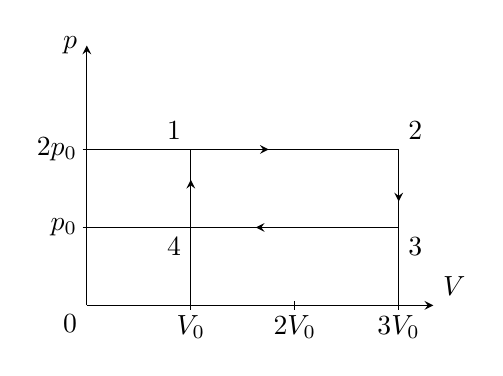
\begin{tikzpicture}[>=stealth,scale=1.1]
\draw[->] (0,0)--(4.0,0) node[above right] {$V$};
\draw[->] (0,0)--(0,3.0) node[left] {$p$};
\node[below left] at (0,0) {$0$};
\draw (0,.9)--(1.2,.9);
\draw (0,1.8)--(1.2,1.8);
\draw (1.2,0)--(1.2,.9);
\draw (3.6,0)--(3.6,.9);
\draw (1.2,.9)--(1.2,1.8)--(3.6,1.8)--(3.6,.9)--cycle;
\draw[->] (1.2,.9)--(1.2,1.45);
\draw[->] (1.2,1.8)--(2.1,1.8);
\draw[->] (3.6,1.8)--(3.6,1.2);
\draw[->] (3.6,.9)--(1.95,.9);
\foreach \x in {1.2,2.4,3.6}\draw (\x,-.05)--(\x,.05);
\foreach \y in {.9,1.8}\draw (-.05,\y)--(.05,\y);
\node[left] at (0,.9) {$p_0$};
\node[left] at (0,1.8) {$2p_0$};
\node[below] at (1.2,0) {$V_0$};
\node[below] at (2.4,0) {$2V_0$};
\node[below] at (3.6,0) {$3V_0$};
\node[above left] at (1.2,1.8) {$1$};
\node[above right] at (3.6,1.8) {$2$};
\node[below right] at (3.6,.9) {$3$};
\node[below left] at (1.2,.9) {$4$};
\end{tikzpicture}
\end{center}
Один моль аргона является рабочим телом в тепловом двигателе, который работает по циклу, показанному на рисунке в переменных $p$--$V$ ($p$ --- давление аргона, $V$ --- его объём).
\begin{enumerate}
\item Аргон получает положительное количество теплоты от нагревателя только в процессе $1$--$2$.
\item В процессе $3$--$4$ внутренняя энергия аргона не изменяется.
\item Работа аргона за цикл равна $2p_0V_0$.
\item В процессе $4$--$1$ аргон отдаёт холодильнику положительное количество теплоты.
\item Максимальная абсолютная температура аргона в цикле в $6$ раз больше минимальной.
\end{enumerate}
}{
\smallskip\noindent\textbf{Решение от GPT}\par
Для одного моля аргона $T=pV/R$, $U=\frac32RT$, $Q=\Delta U+A$.
\begin{enumerate}
\item Неверно: теплота поступает на $1$--$2$ и на $4$--$1$; в обоих процессах температура растёт.
\item Неверно: на $3$--$4$ произведение $pV$ уменьшается, поэтому $\Delta U<0$.
\item Верно: работа за цикл равна площади прямоугольника, $A_{\text{ц}}=(2p_0-p_0)(3V_0-V_0)=2p_0V_0$.
\item Неверно: на $4$--$1$ объём постоянен, температура растёт, поэтому $Q=\Delta U>0$.
\item Верно: максимальная температура достигается в точке $2$, минимальная --- в точке $4$; $T_2/T_4=(2p_0\cdot3V_0)/(p_0V_0)=6$.
\end{enumerate}
\textbf{Ответ: 35.}
}

% Source 25384: https://phys-ege.sdamgia.ru/problem?id=25384
\BankTask{25384}{
\begin{center}\begin{tikzpicture}[task graph,>=stealth]\draw[->](0,0)--(5,0)node[below]{\(V\)};\draw[->](0,0)--(0,3.7)node[left]{\(p\)};\node[below left]at(0,0){\(0\)};\fill(1,0.85)circle(1.25pt)node[below left]{\(1\)};\fill(1,3.05)circle(1.25pt)node[above left]{\(2\)};\fill(3.85,0.85)circle(1.25pt)node[below right]{\(3\)};\draw(1,0.85)--(1,3.05);\draw[->](1,0.85)--(1.000,2.214);\draw(3.85,0.85)--(1,0.85);\draw[->](3.85,0.85)--(2.083,0.850);\draw(1,3.05)..controls(1.45,1.95)and(2.55,1.58)..(3.85,.85);\draw[->](1.9,1.91)--(2.2,1.72);\end{tikzpicture}\end{center}
$1$ моль одноатомного идеального газа совершает цикл $1$–$2$–$3$–$1$, состоящий из изохоры ($1$–$2$), адиабаты ($2$–$3$) и изобары ($3$–$1$). Абсолютные температуры газа $T_{1}$  =  $400$ K, $T_{2}$  =  $600$ K, $T_{3}$  =  $510$ K. Определите КПД цикла.
}{
\smallskip\noindent\textbf{Решение}\par
КПД циклического процесса равно $\eta = \frac{A}{Q_{\,\text{пол}}} .$ Найдем работу за цикл $A=A_1{,}2 + A_2{,}3 + A_3{,}1.$ Для изохорного процесса $A_1{,}2=0.$ При адиабатном процессе из первого закона термодинамики $Q_2{,}3=A_2{,}3 + \Delta U_2{,}3$ следует, что $A_2{,}3= - \Delta U_2{,}3,$ так как $Q_2{,}3=0,$ а изменение внутренней энергии $\Delta U_2{,}3= \frac{3}{2} \nu R ( T_3 - T_2 ) .$ Для изобарного процесса $A_3{,}1=p\Delta V.$ Учитывая, что из уравнения Клапейрона  — Менделеева $pV=\nu RT,$ то $A_3{,}1=\nu R ( T_1 - T_3 ) .$ Таким образом, работа газа за цикл:

\[A=\nu R ( \frac{3}{2} ( T_2 - T_3 ) + ( T_1 - T_3 ) ) .\]

Из графика следует, что при изохорном процессе газ получал теплоту, при адиабатном процессе количество теплоты равно $0$, при изобарном процессе газ теплоту отдавал. Значит, необходимо найти количество теплоты при изохорном процессе. Из первого закона термодинамики $Q_1{,}2=A_1{,}2 + \Delta U_1{,}2,$ но при этом $A_1{,}2=0,$ а $\Delta U_1{,}2= \frac{3}{2} \nu R ( T_2 - T_1 ) ,$ то от нагревателя получена теплота $Q_{\,\text{пол}}= \frac{3}{2} \nu R ( T_2 - T_1 ) .$
Тогда КПД цикла:

\[\eta = \frac{\frac{3}{2} ( T_2 - T_3 ) + ( T_1 - T_3 )}{\frac{3}{2} ( T_2 - T_1 )} = \frac{1{,}5 \cdot ( 600 - 510 ) + ( 400 - 510 )}{1{,}5 \cdot ( 600 - 400 )} \approx 0{,}08=8\% .\]

Ответ: $8$\%.
}

% Source 43206: https://phys-ege.sdamgia.ru/problem?id=43206
\BankTask{43206}{
\begin{center}\begin{tikzpicture}[task graph,>=stealth]\draw[->](0,0)--(5,0)node[below]{\(V\)};\draw[->](0,0)--(0,3.7)node[left]{\(p\)};\node[below left]at(0,0){\(0\)};\fill(0.7,3)circle(1.25pt)node[above]{\(1\)};\fill(3.15,3)circle(1.25pt)node[above right]{\(2\)};\fill(3.15,0.47)circle(1.25pt)node[right]{\(3\)};\draw(.7,3)--(3.15,3)--(3.15,.47)..controls(1.38,.55)and(.82,1.5)..(.7,3);\end{tikzpicture}\end{center}
Один моль одноатомного идеального газа совершает цикл $1$–$2$–$3$–$1$, состоящий из изобары ($1$–$2$), изохоры ($2$–$3$) и адиабаты ($3$–$1$). Абсолютные температуры газа в состояниях $1$, $2$ и $3$ равны $400$ К, $800$ К и $252$ К соответственно. Определите КПД теплового двигателя, работающего по этом циклу.
}{
\smallskip\noindent\textbf{Решение}\par
На участке $1$−$2$ при изобарном расширении температура газа также увеличивается согласно закону $\frac{V}{T} =const.$ При этом газ совершает положительную работу $A_{12}=\nu R ( T_2 - T_1 ) ,$ его внутренняя энергия увеличивается $\Delta U_{12}= \frac{3}{2} \nu R ( T_2 - T_1 ) .$ Согласно первому закону термодинамики газ получает от нагревателя количество теплоты

\[Q_{12}=A_{12} + \Delta U_{12}= \frac{5}{2} \nu R ( T_2 - T_1 ) .\]

На участке $2$−$3$ давление изохорно уменьшается. Согласно закону $\frac{p}{T} =const$ температура газа уменьшается. Тогда газ работу не совершает, а его внутренняя энергия уменьшается $\Delta U_{23}= \frac{3}{2} \nu R ( T_3 - T_2 ) .$ По первому закону термодинамики газ отдает холодильнику количество теплоты

\[|Q_{23}|=A_{23} + \Delta U_{23}= \frac{3}{2} \nu R|T_3 - T_2|= \frac{3}{2} \nu R ( T_2 - T_3 ) .\]

Процесс $3$−$1$ является адиабатным, поэтому $Q_{31}=0.$
Тогда КПД теплового двигателя:

\[\eta=1 - \frac{Q_{\,\text{х}}}{Q_{\,\text{н}}} =1 - \frac{|Q_{23}|}{Q_{12}} =1 - \frac{3 ( T_2 - T_3 )}{5 ( T_2 - T_1 )} =1 - \frac{3 \cdot ( 800 - 252 )}{5 \cdot ( 800 - 400 )} =0{,}178=17{,}8\%.\]

Ответ: $17{,}8$\%.
}

% Source 35344: https://phys-ege.sdamgia.ru/problem?id=35344
\BankTask{35344}{
\begin{center}\begin{tikzpicture}[task graph,>=stealth]\draw[gray!65,step=.8] (0,0) grid (4,3.2);\draw[->](0,0)--(5,0)node[below]{\(V\)};\draw[->](0,0)--(0,3.7)node[left]{\(p\)};\node[below left]at(0,0){\(0\)};\fill(0.8,0.8)circle(1.25pt)node[below left]{\(1\)};\fill(0.8,1.6)circle(1.25pt)node[above left]{\(2\)};\fill(3.2,2.4)circle(1.25pt)node[above right]{\(3\)};\draw(0.8,0.8)--(0.8,1.6);\draw[->](0.8,0.8)--(0.800,1.296);\draw(0.8,1.6)--(3.2,2.4);\draw[->](0.8,1.6)--(2.288,2.096);\draw(3.2,2.4)--(0.8,0.8);\draw[->](3.2,2.4)--(1.712,1.408);\node[left]at(0,.8){\(p_0\)};\node[left]at(0,2.4){\(3p_0\)};\node[below]at(.8,0){\(V_0\)};\node[below]at(3.2,0){\(4V_0\)};\end{tikzpicture}\end{center}
В цикле, показанном на pV-диаграмме, v  =  $4$ моль разреженного гелия получает от нагревателя количество теплоты $Q_{\,\text{нагр}}$  =  $120\,\text{кДж}$. Найдите температуру $T_{2}$ гелия в состоянии $2$.
}{
\smallskip\noindent\textbf{Решение}\par
Согласно графику цикла гелий получает положительное количество теплоты от нагревателя на участках $1$−$2$ и $2$−$3$. При этом процесс $1$–$2$ является изохорным и газ работы не совершает. 
По первому закону термодинамики для процесса $1$–$2$ $Q_1{,}2=\Delta U_1{,}2,$ изменение внутренней энергии в этом процессе:

\[\Delta U_1{,}2=U_2 - U_1= \frac{3}{2} p_0V_0.\]

Для процесса $2$–$3$ по первому закону термодинамики $Q_2{,}3=\Delta U_2{,}3 + A_2{,}3.$ Изменение внутренней энергии для данного процесса:

\[\Delta U_2{,}3=U_3 - U_2= \frac{3}{2} ( 12p_0V_0 - 2p_0V_0 ) =15p_0V_0.\]

Работу газа для процесса $2$–$3$ найдем графически как площадь фигуры под графиком:

\[A_2{,}3= \frac{p_2 + p_3}{2} ( V_3 - V_2 ) = \frac{2p_0 + 3p_0}{2} ( 4V_0 - V_0 ) = \frac{15}{2} p_0V_0.\]

Тогда полученное количество теплоты равно: 

\[Q_{\max p} =Q_{12} + Q_{23} = \frac{3}{2} p_0V_0 + 15p_0V_0 + \frac{15}{2} p_0V_0 =24 p_0 V_0 .\]

Согласно графику цикла $v R T_2=2 p_0 V_0,$ откуда: 

\[T_2= \frac{2 p_0 V_0}{v R} = \frac{Q_{\,\text{нагр}}}{12 v R} = \frac{120 \cdot 10 ^3}{12 \cdot 4 \cdot 8{,}31} =301 \,\text{К} .\]

Ответ: $301$ К.
}

\end{document}
